\documentclass{article}
\usepackage{graphicx}

\begin{document}
\section{Results}
To be sure about the quality of the juxtacellular recording, auto-correlograms were computed for each recording (Fig. \ref{fig:AC}).
\begin{figure}[!h]
	\centering
	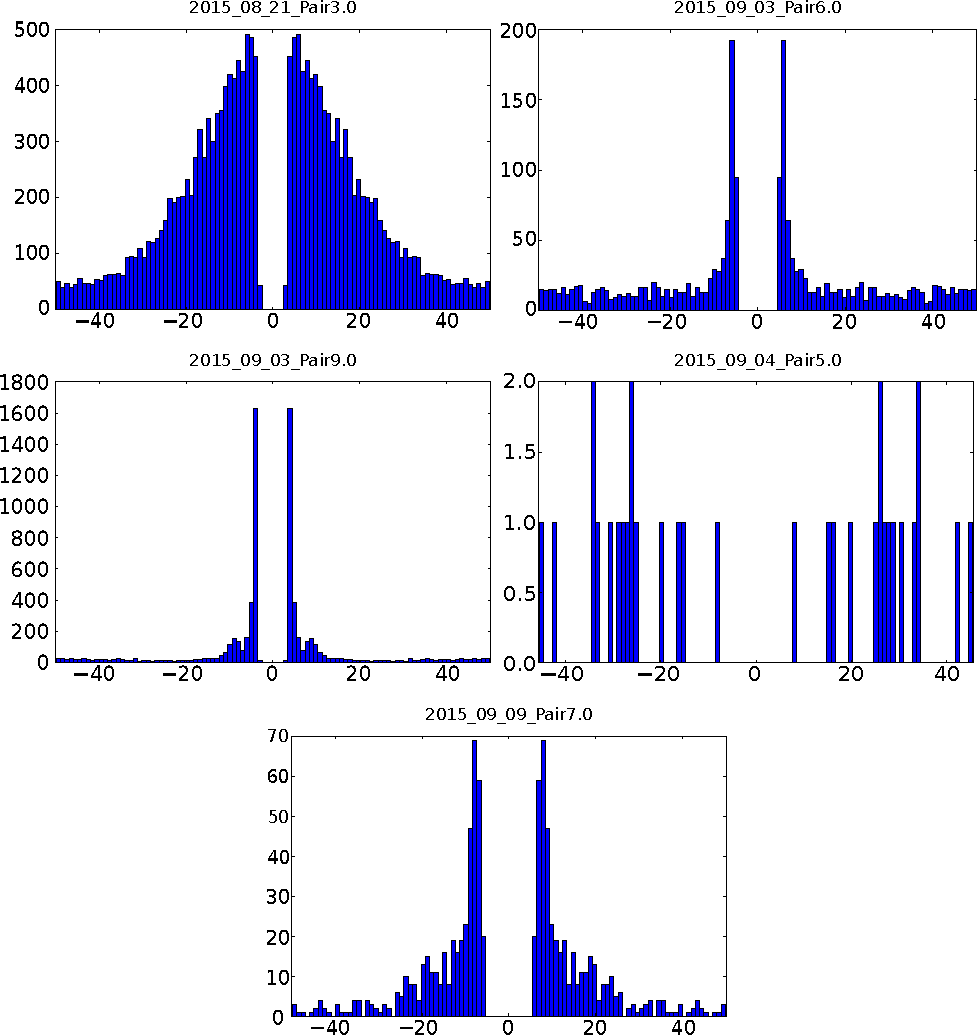
\includegraphics[width=\linewidth]{AC.pdf}
	\caption{Auto-Correlograms for all the recordings. The size of the bins in the histograms is 1 ms and the value for the lag is 50ms.
}
\label{fig:AC}
\end{figure}

All the auto-correlograms display a usual distribution, clearly showing a gap in the interval from -5ms to 5ms, assuring that the cell never spiked twice  within a 5ms interval, which conforms with the typical values of refractory period of 2-3ms.

It is worth noting that on the auto-correlogram corresponding to the recording 939 a second peak is resolved around $\tau = -9 ms$ and $\tau = 9 ms$.

For each recording, phy was run with the following parameters:
The data was filtered with a forwards-backwards Butterworth filter of order 3 with cutoff frequency set to 500Hz. The noise standard deviation was evaluated in 50 excerpts of 1 second each. The weak threshold was $\theta_w = 2 \sigma_{noise}$ and the strong threshold was $\theta_s = 4.5 \sigma_{noise}$.

The results are presented in table \ref{tab:results-from-phy}.

\begin{table}[!h]

\begin{center}
\begin{tabular}{ccccc}
Recording ID & \# detected Spikes & $\sigma_{noise}$ ($\mu V$) & $\theta_W$ ($\mu V$) & $\theta_S$ ($\mu V$) \\ \hline
8213 & 148762 &  12.95 & 25.91 & 58.30 \\ 
936 & 323629 & 10.76 & 21.52 & 48.43 \\ 
939 & 265476 & 10.51 & 21.02 & 47.29 \\ 
945 & 126234 & 10.92 & 21.84 & 49.14 \\ 
997 & 156932 & 11.47 & 22.93 & 51.60 \\ 
\end{tabular}
\end{center}
\caption{Summary of the output from phy. In this table are the values of the estimated standard deviations of the noise, and the calculated weak and strong thresholds for each recording. These values were converted into $\mu V$.}
\label{tab:results-from-phy}
\end{table}

In Fig. \ref{fig:CC} are the whole-probe cross-correlograms for the recordings, where for each detected spike, all electrodes whose corresponding mask value was non-zero were used.

\begin{figure}[!h]
	\centering
	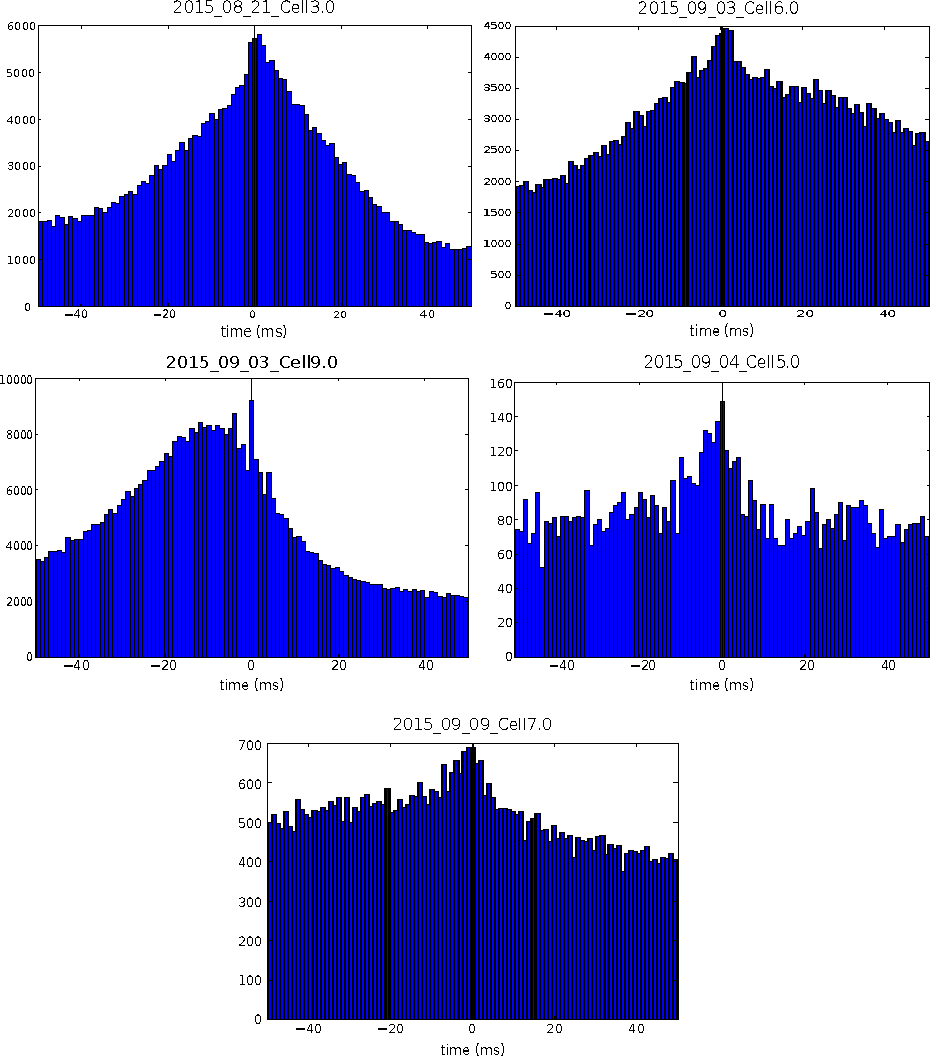
\includegraphics[width=\linewidth]{CC.pdf}
	\caption{Cross-Correlograms for all the recordings. The size of the bins in the histograms is 1 ms and the value for the lag is 50ms.
}
\label{fig:CC}
\end{figure}

In Appendix NUMBEROFAPPENDIX are the cross-correlograms per channel, where the spike train output by phy was split according to the electrode the spike was detected on using the masks.

On Fig \ref{fig:CC}, all cross-correlograms present a somewhat coherent distribution. This means that for every value $\tau$ in the considered interval, there exists some temporal correlation between the juxta neuron and the activity of the rest of the neurons in the recorded volume. This is to be expected. According to Ruiz-Mejias et al., the use of ketamine as anesthesia in rats provokes the synchronization in the population activity in many cortical areas, including the motor cortex. This gives rise to "up" and "down" states, where most neurons in the population are firing or silent, respectively. In addition, they report that the frequency of oscillation of these states is, on average, 0.97Hz, which is close to the firing rates observed in the juxtacellular recordings from Neto et al. 

Only on the cross-correlogram corresponding to the recording 939 can we see a distinct peak when $\tau=0 ms$, on top of the correlation with the background activity. This means that phy managed to find juxta neuron.

On the rest of the cross-correlograms in Fig \ref{fig:CC}, the peak around the central bin is never very clear. In fact, in the case of the recordings 8213 and 936, the peak is even shifted to $\tau=1 ms$. This could justify a more careful examination setting the size of the bin used in the histograms to a smaller value.

To calculate the number of events corresponding to the juxta, it is necessary to remove the counts from the correlation with the background activity. To estimate this value, the average of the counts in the bin neighboring bins ($\tau = -1ms$ and $\tau = 1 ms$) was computed and subtracted to the counts in the central bin. The results are in table \ref{tab:CCcorrection}.

\begin{table}[!h]
\begin{center}
\begin{tabular}{p{1.5cm}|c|c|c|p{1.3cm}|c|r}

\multicolumn{ 1}{p{1.5cm}|}{Recording ID} & \multicolumn{ 3}{c|}{Bin Counts} &  \multicolumn{ 1}{p{1.3cm}|}{Corrected Counts} & \multicolumn{ 1}{c|}{\#juxtaSpikes} & \multicolumn{ 1}{c}{Accuracy} \\ 
\multicolumn{ 1}{c|}{} & $\tau=0$ & $\tau=-1$ & $\tau=1$ & \multicolumn{ 1}{c|}{} & \multicolumn{ 1}{p{1.3cm}|}{} & \multicolumn{ 1}{l}{} \\ \hline
8213 & 5725 & 5642 & 5810 & -1 & 7760 & -0.01\% \\ \hline
936 & 4377 & 4357 & 4465 & -34 & 3329 & -1.02\% \\ \hline
939 & 9202 & 6701 & 7092 & 2305.5 & 4947 & 46.60\% \\ \hline
945 & 144 & 137 & 120 & 15.5 & 185 & 8.38\% \\ \hline
997 & 691 & 689 & 650 & 21.5 & 1082 & 1.99\% \\ \hline
\end{tabular}
\end{center}
\caption{Correction of the cross-correlograms central peak.}
\label{tab:CCcorrection}
\end{table}

Even in the recording 939 the detection rate is fairly low, considering it has a very large P2P amplitude.
In the other cases, phy yields a detection accuracy close to zero. This is not surprising considering the algorithm used by phy. The maximum P2P amplitude of JTAs of these case lies between lies between 19.4$\mu V$ and 30.8$\mu V$ and the strong threshold is always larger than 48.43 $\mu V$. Since it is required that at least one sample in a connected component be larger than the strong threshold these spikes are never detected. Two possible explanations exist for this number of detected events. First, the neuron may have spiked simultaneously to a large noise fluctuation causing it to be detected. Secondly, the connected components of these spikes could have been connected with the connected component of other spike which exceeded the strong threshold. This would result in the detection one single spike where the computed spike time was closer to the corresponding juxta spike time and therefore contributed to the central bin in the cross-correlograms.


\end{document}